\documentclass[12pt]{article}
\usepackage[
    a4paper,
    top=0.5in,
    bottom=0.5in,
    left=1in,
    right=1in,
    headheight=22pt,
    headsep=3em,
    includeheadfoot
]{geometry}
\usepackage{amssymb,amsmath}
\usepackage{parskip}
\usepackage{fancyhdr}
\usepackage{tabularx}
\usepackage{enumerate}
\usepackage{graphicx}
\usepackage{tikz}
\usepackage{array}
\usepackage{cmbright}

% commands
\renewcommand{\headrulewidth}{0mm}

\newcommand{\HomeworkNo}{1}
\newcommand{\MyName}{Amy M. Liu}
\newcommand{\MyPennKey}{liuamy05}
\newcommand{\PrintFirstHeader}{
    \begin{center}
    {\LARGE{\textbf{Homework \HomeworkNo{}}}} \vspace{0.5em} \\
    PennKey: \MyPennKey \\
    Collaborators: Hugo Song
    \end{center}
    \vspace{1em}
}
%%%

% fancyhdr
\pagestyle{fancy}
\fancyhead[L]{\MyName}
\fancyhead[R]{Homework \HomeworkNo{}}
\fancypagestyle{firstpage}{
    \fancyhead[L]{CIS 2620 Summer 2025}
    \fancyhead[R]{\Large{\MyName}}
}
%%%

% customizations
\newcolumntype{C}{>{$}c<{$}}
\usetikzlibrary{automata, positioning, arrows}
\tikzset{
    auto,
    on grid,
    initial text=$ $,
    shorten >=1pt,
    node distance=2cm,
    accepting/.style={fill=red!25, double},
}
%%%

\begin{document}
\thispagestyle{firstpage}
\PrintFirstHeader{}
\begin{enumerate}[\bf P1.]
\setlength\itemsep{1em}

\item
The given language is:
\[
\mathbb{L} = \{x \in \{0,1\}^* : \text{ the number of occurrences of 01 in x is same as that of 10}\} \\
\]

We will define our DFA in the following form:
\[
\mathbb{M} = \{\mathbb{Q}, \Sigma, \delta, q_0, \mathbb{F}\}
\]

The respective variables are:
\[
\begin{aligned}
\mathbb{Q} :=& \{ q_0, q_1, q_2, q_3, q_4\} \\
\Sigma :=& \{0, 1\} \\
q_0 :=& q_0 \\
\mathbb{F} :=& \{q_0, q_1, q_2\} \\
\end{aligned}
\]

The transition function is laid out below:
\begin{figure}[ht]
\centering
\begin{tabular}{ C | C C }
    \multicolumn{3}{C}{\boldsymbol{\delta := \delta(q, \sigma) : \mathbb{Q} \times \Sigma}} \\
    \hline
    \textbf{q} & \boldsymbol{\delta : \sigma = 0} & \boldsymbol{\delta : \sigma = 1} \\
    q_0 & q_1 & q_2 \\
    q_1 & q_1 & q_3 \\ 
    q_2 & q_4 & q_2 \\
    q_3 & q_1 & q_3 \\
    q_4 & q_4 & q_2 \\
\end{tabular}
\end{figure}

\textbf{Overall DFA diagram:}
\begin{figure}[ht]
    \centering
    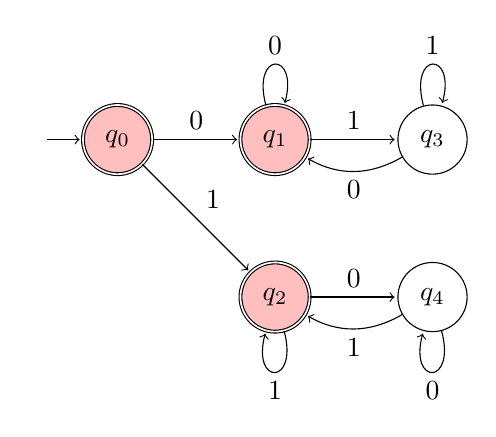
\begin{tikzpicture}
        \node[state, accepting, initial] (q0) {$q_0$};
        \node[state, accepting, right of=q0] (q1) {$q_1$};
        \node[state, accepting, below of=q1] (q2) {$q_2$};
        \node[state, right of=q1] (q3) {$q_3$};
        \node[state, below of=q3] (q4) {$q_4$};

    \path[->]
        (q0) edge node[above] {0} (q1)
            edge node {1} (q2)
        (q1) edge[loop above] node {0} ()
            edge node {1} (q3)    
        (q2) edge node {0} (q4)
            edge[loop below] node {1} ()
        (q3) edge[loop above] node {1} ()
            edge[bend left] node {0} (q1) 
        (q4) edge[loop below] node {0} ()
            edge[bend left] node {1} (q2);
    \end{tikzpicture}
\end{figure}

\newpage
\item
The given language is:
\[
\mathbb{L} = \{x \in \{0,1\}^* : x \text{ starts with a 11 and ends with 11 and } |x| \geq 3\} \\
\]

To prove that the language is regular, we define a DFA, $\mathbb{M} = \{\mathbb{Q}, \Sigma, \delta, q_0, \mathbb{F}\}$, as follows:
\[
\begin{aligned}
\mathbb{Q} :=& \{ q_0, q_1, q_2, q_3, q_4, q_5, q_6, q_{sink}\} \\
\Sigma :=& \{0, 1\} \\
q_0 :=& q_0 \\
\mathbb{F} :=& \{q_6\} \\
\end{aligned}
\]

Transition function $\delta$:
\begin{figure}[ht]
\centering
\begin{tabular}{ C | C C }
    \multicolumn{3}{C}{\boldsymbol{\delta := \delta(q, \sigma) : \mathbb{Q} \times \Sigma}} \\
    \hline
    \textbf{q} & \boldsymbol{\delta : \sigma = 0} & \boldsymbol{\delta : \sigma = 1} \\
    q_0 & q_{sink} & q_1 \\
    q_1 & q_{sink} & q_2 \\ 
    q_2 & q_3 & q_6 \\
    q_3 & q_4 & q_5 \\
    q_4 & q_4 & q_5 \\
    q_5 & q_3 & q_6 \\
    q_6 & q_3 & q_6 \\
    q_{sink} & q_{sink} & q_{sink} \\
\end{tabular}
\end{figure}

\textbf{Overall DFA diagram:}
\begin{figure}[ht]
    \centering
    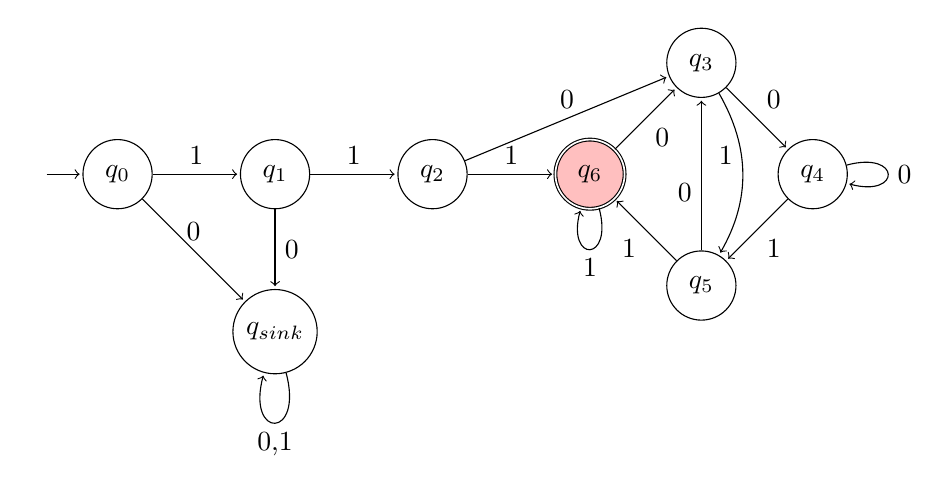
\begin{tikzpicture}
        \node[state, initial] (q0) {$q_0$};
        \node[state, right of=q0] (q1) {$q_1$};
        \node[state, right of=q1] (q2) {$q_2$};
        \node[state, accepting, right of=q2] (q6) {$q_6$};
        \node[state, above right of=q6] (q3) {$q_3$};
        \node[state, below right of=q3] (q4) {$q_4$};
        \node[state, below left of=q4] (q5) {$q_5$};
        \node[state, below of=q1] (qsink) {$q_{sink}$};

    \path[->]
        (q0) edge node[above] {0} (qsink)
            edge node {1} (q1)
        (q1) edge node {0} (qsink)
            edge node {1} (q2)
        (q2) edge node[above] {0} (q3)
            edge node {1} (q6)
        (q3) edge node {0} (q4)
            edge[bend left] node[above left] {1} (q5)
        (q4) edge [loop right] node {0} (q4)
            edge node {1} (q5)
        (q5) edge node[below left] {0} (q3)
            edge node {1} (q6)
        (q6) edge node[below right] {0} (q3)
            edge[loop below] node {1} ()
        (qsink) edge [loop below] node {0,1} ();
    \end{tikzpicture}
\end{figure}

\textbf{Proof of Correctness:}

We want to justify that $\mathbb{L}(\mathbb{M}) = \mathbb{L}$. We can do so with a bidirectional proof:
\[ 
\mathbb{M} \text{ accepts a string } x \Leftrightarrow{} x \in \mathbb{L}
\]
\textbf{($\Rightarrow$)} If $\mathbb{M}$ accepts a string x, x $\in \mathbb{L}$

If x was accepted, we know there exists an accepting path of states:
\[
q_0 \xrightarrow{x_1} p^{(1)} \xrightarrow{x_2} p^{(2)} \xrightarrow{\cdots} \cdots \xrightarrow{x_{n-1}} p^{(n-1)} \xrightarrow{x_n} p^{(n)}
\]
Assume, for the sake of contradiction, that $x_1 = 0$. This would mean $p^{(1)} = q_{sink}$. However, since this is an accepting path, $p^{(n)} = q_6$. Since $\delta(q_{sink}, \sigma) = q_{sink}$ no matter the input $\sigma$, it would be impossible for the path to arrive at $q_6$. Thus, $x_1$ must be 1.

Similarly, if $x_2 = 0$, $p^{(2)} = q_{sink}$, which contradicts our accepting path principles. So $x_2$ also equals 1.

We have just proven that $x_{1}=1$ and $x_2=1$, so x must begin with 11.

Now, we can look at $x_n$. Again, assume that $x_n$ = 0. However:
\[
\forall q \in \mathbb{Q}, \delta(q, 0) \neq q_6
\]
This means that no state can transition into $q_6$ w/ an input 0, and $p^{(n)} = q_6$ is a contradiction. So $x_n = 1$.

Lastly, if $x_n = 1$, we can refer to our transition function to see that $p^{(n-1)} = q_2 \| q_5$.

\begin{itemize}
    \item Case $q_2$: To arrive at $q_2$, $x_{n-1}$ must be 1 (due to $q_{sink}$ causing the same contradictions as explained above).
    \item Case $q_5$: If $\delta(q, \sigma) = q_5$, we can see $\sigma = 1$ for all possible cases of q ($q_3, q_4$). So $x_{n-1}$ must be 1.
\end{itemize}

We have just proven that $x_{n-1}=1$ and $x_n=1$, so x must end with 11.

Thus, if $\mathbb{M}$ accepts a string x, x $\in \mathbb{L}$.

\vspace{1.5em}

\textbf{($\Leftarrow$)} If a string x $\in \mathbb{L}$, $\mathbb{M}$ accepts x.

If x $\in \mathbb{L}$, we know it must begin and end with 1, and have length greater than 3. 

If $|x| = 3$, x = 111. If we input this into $\mathbb{M}$, we get this path:
\[
q_0 \xrightarrow{1} q_1 \xrightarrow{1} q_2 \xrightarrow{1} q_6
\]
If $|x| = 4$, x = 1111. If we input this into $\mathbb{M}$, we get this path:
\[
q_0 \xrightarrow{1} q_1 \xrightarrow{1} q_2 \xrightarrow{1} q_6 \xrightarrow{1} q_6
\]
If $|x| > 4$, x has the following form:
\[
x = 1 1 ... x_{n-2} 1 1
\]
and there must exist a path:
\[
q_0 \xrightarrow{1} q_1 \xrightarrow{1} q_2 \xrightarrow{\cdots} \cdots \xrightarrow{x_{n-2}} p^{(n-2)} \xrightarrow{1} p^{(n-1)} \xrightarrow{1} p^{(n)}
\]
Let's look at the possible states for $p^{(n-2)}$. 

\begin{itemize}
    \item $p^{(n-2)} \neq q_0 \| q_1 \| q_{sink}$. This is because we have already arrived at $q_2$, and no path leading out of $q_2$ can ever arrive back at $q_0 \| q_1 \| q_{sink}$.
    \item If $p^{(n-2)} = q_2 \| q_5 \| q_6$,  we refer to our transition function and known input x-values in the path above to see that $p^{(n-1)} = q_6$ and $p^{(n)} = q_6$. x is correctly accepted by $\mathbb{M}$.
    \item If $p^{(n-2)} = q_3 \| q_4$,  we follow similar logic as the above case to see that  $p^{(n-1)} = q_5$ and $p^{(n)} = q_6$. x is correctly accepted by $\mathbb{M}$.
\end{itemize}

Since these cover all the possible cases for $p^{(n-2)}$, we know that our string x (length greater than 4) will always be accepted by $\mathbb{M}$. Now we've also covered all lengths of x, so we've shown that if a string x $\in \mathbb{L}$, $\mathbb{M}$ accepts x.

\newpage
\item

To prove that any DFA for $\mathbb{L}$ must have at least $2^k$ states, it is sufficient to find $2^k$ strings $x_{(1)}, \dots, x_{(2^k)}$ s.t. for any i $\neq$ j, $x_{(i)}$ and $x_{(j)}$ are distinguishable w.r.t. $\mathbb{L}$.

To begin, let $\Sigma = \{\sigma_1, \sigma_2, \cdots, \sigma_k\}$.

We propose that the $2^k$ strings correspond to the power set of $\Sigma$, i.e. the set of all subsets of $\Sigma$. As in, for a given subset $S \subseteq \Sigma$, the corresponding string $x_{S}$ is created by listing the elements in $S$ (to make this even more well-defined, we establish an arbitrary total order on $\Sigma$, and list the elements in increasing order). If the subset is the empty set, $x_S = \varepsilon$, the empty string.

Based on the fact that we constructed each $x_S$ from a subset $S$ of $\Sigma$, which by definition cannot contain an element of $\Sigma$ more than once, we know that $x_S$ must also be a string in which each symbol occurs exactly once, so $x_S \in \mathbb{L}$.

Furthermore, as mentioned, we create a string for each possible subset of $\Sigma$, which is exactly the power set $P$. $|\Sigma| = k$, so $|P(\Sigma)| = 2^k$, and we have constructed $2^k$ strings.

We will prove that these $2^k$ strings are distinguishable with respect to L.

Let $A \neq B \subseteq \Sigma$. Then there exists a symbol $\sigma \in \Sigma$ such that $\sigma \in A \backslash B$ or $\sigma \in B \backslash A$.

Without loss of generality, suppose $\sigma \in A \backslash B$.

Now, consider the subsets' corresponding strings: $x_A$ and $x_B$, and let z = $\sigma$

\begin{itemize}
    \item $x_A z$ must contain two copies of $\sigma$, since $\sigma \in$ A, and $x_A$ was constructed from A. So $x_A z \notin \mathbb{L}$.
    \item $x_B z$ contains $\sigma$ only once, since $\sigma \notin$ B. So $x_A z \in \mathbb{L}$.
\end{itemize}

Hence, $x_A$ and $x_B$ are distinguishable with respect to $\mathbb{L}$. This will work for every pair of subsets $A \neq B$. Looking at the set of strings $\{x_S : S \subseteq \Sigma\}$, we have successfully constructed $2^k$ pairwise distinguishable strings w/ respect to $\mathbb{L}$.

\newpage
\item
The given language is:
\[
\mathbb{L} = \{x \in \Sigma^* : \text{ there exists a symbol which appears in x more than once}\} \\
\]

We will define our NFA in the following form:
\[
\mathbb{N} = \{\mathbb{Q}, \Sigma, \Delta, q_0, \mathbb{F}\}
\]

The respective variables are:
\[
\begin{aligned}
\mathbb{Q} :=& \{ q_0, q_1, \cdots q_k, q_{accept}\} \\
\Sigma :=& \{\sigma_1 \cdots \sigma_k\} \\
q_0 :=& q_0 \\
\mathbb{F} :=& \{q_{accept}\} \\
\end{aligned}
\]

The transition function is laid out below:
\begin{figure}[ht]
\centering
\begin{tabular}{ C C C }
    \multicolumn{3}{C}{\boldsymbol{\Delta := \Delta(q, \sigma) : \mathbb{Q} \times \Sigma \rightarrow 2^{Q}}} \\
    \hline
    \textbf{q} & \boldsymbol{\sigma} & \boldsymbol{\Delta} \\
    q_0 & \sigma_i \text{ (any $i$)} & \{q_0, q_i\} \\
    q_i & \sigma_i & \{q_{accept}\} \\
    q_i & \sigma \neq \sigma_i & \{q_i\} \\
    q_{accept} & \text{any } \sigma & \{q_{accept}\} \\
\end{tabular}
\end{figure}

\textbf{Explanation of $\Delta$:}
\begin{description}
\item[\textbf{Row 1}\,: \(\Delta(q_0,\sigma_i)=\{q_0,q_i\}\).] 
        When the start state \(q_0\) reads some symbol \(\sigma_i\), $\mathbb{N}$ \textit{nondeterministically} starts two "threads", (i) stays in \(q_0\), the scanning state, and (ii) “chooses” \(\sigma_i\) as the candidate $\sigma$ that will be repeated and moves to state \(q_i\).

\item[\textbf{Row 2}\,: \(\Delta(q_i,\sigma_i)=\{q_{\text{accept}}\}\).] 
        While in \(q_i\) we have already seen \emph{exactly one} copy of \(\sigma_i\).  
        Reading a second \(\sigma_i\) confirms the language condition,
        so we transition to the accepting state \(q_{\text{accept}}\).

\item[\textbf{Row 3}\,: \(\Delta(q_i,\sigma\neq\sigma_i)=\{q_i\}\).] 
        Any symbol other than \(\sigma_i\) is irrelevant to the current
        guess, so $\mathbb{N}$ remains in \(q_i\) and continues waiting
        for the repeat of \(\sigma_i\).

\item[\textbf{Row 4}\,: \(\Delta(q_{\text{accept}},\sigma)=\{q_{\text{accept}}\}\) for any \(\sigma\).] 
        Once \(q_{\text{accept}}\) is reached, the string x is already known to contain a repeated symbol. The run therefore stays in this accepting state for the rest of the input.
\end{description}

\vspace{1em}

\textbf{Proof of Correctness:}

We show that $\mathbb{N}$ accepts input string x \textit{iff} there exists a symbol which appears in x more than once.

\textbf{($\Rightarrow$)}
Assume $\mathbb{N}$ accepts $x$. Acceptance implies that some computation of $\mathbb{N}$ ends in $q_{\text{accept}}$. By the definition of $\Delta$, the \textit{only} transition into
$q_{\text{accept}}$ is:
\[
  q_i \xrightarrow{\sigma_i} q_{\text{accept}}
\]
for some $i$. Entering $q_i$ earlier means one $\sigma_i$ had already been read (Row 1 of the table), and the transition above consumes a \textit{second} $\sigma_i$ (Row 2). Thus $\sigma_i$ occurs at least twice in $x$.

\textbf{($\Leftarrow$)}
Conversely, suppose $x$ contains a symbol $\sigma_i$ that appears at least twice. Looking at $\mathbb{N}$ we can see that there will always be a thread that stays in $q_0$ until the first occurrence of $\sigma_i$; then, that thread takes the nondeterministic branch to $q_i$ (Row 1). Because $\sigma_i$ occurs again in $x$, the later $\sigma_i$ triggers $q_i\xrightarrow{\sigma_i}q_{\text{accept}}$ (Row 2). Row 4 keeps $\mathbb{N}$ in $q_{accept}$ for the rest of the input, so this computation accepts $x$.

\vspace{1em}

Since both directions hold, $\mathbb{L}(\mathbb{N})$ is exactly the language:
\[
\mathbb{L} = \{x \in \Sigma^* : \text{ there exists a symbol which appears in x more than once}\} \\
\]
Furthermore, the construction uses $1$ start state $q_0$, $k$ intermediate states $q_i$ ($i=1,\dots,k$),
and $1$ accepting state $q_{\text{accept}}$,
for a total of $k+2\le 2k+2$ states, satisfying the required limit.


\end{enumerate}
\end{document}